%%%%%%%%%%%%%%%%%%%%%%%%%%%%%%%%%%%%%%%%%%%%%%%%%%%%%%%%%%%%
%%% ELIFE ARTICLE TEMPLATE
%%%%%%%%%%%%%%%%%%%%%%%%%%%%%%%%%%%%%%%%%%%%%%%%%%%%%%%%%%%%
%%% PREAMBLE 
\documentclass[9pt,lineno]{elife}
% Use the onehalfspacing option for 1.5 line spacing
% Use the doublespacing option for 2.0 line spacing
% Please note that these options may affect formatting.
% Additionally, the use of the \newcommand function should be limited.


\usepackage{lipsum} % Required to insert dummy text
\usepackage[version=4]{mhchem}
\usepackage{siunitx}
\DeclareSIUnit\Molar{M}

%%%%%%%%%%%%%%%%%%%%%%%%%%%%%%%%%%%%%%%%%%%%%%%%%%%%%%%%%%%%
%%% ARTICLE SETUP
%%%%%%%%%%%%%%%%%%%%%%%%%%%%%%%%%%%%%%%%%%%%%%%%%%%%%%%%%%%%
\title{Single-cell virus sequencing of influenza variants that trigger innate immunity}

\author[1]{Alistair B. Russell}
\author[1,2,3*]{Jesse D. Bloom}
\affil[1]{Basic Sciences Division and Computational Biology Program, Fred Hutchinson Cancer Research Center, Seattle, United States}
\affil[2]{Department of Genome Sciences, University of Washington, Seattle, United States}
\affil[3]{Howard Hughes Medical Institute, Fred Hutchinson Cancer Research Center, Seattle, United States}

\corr{jbloom@fredhutch.org}{JDB}

%%%%%%%%%%%%%%%%%%%%%%%%%%%%%%%%%%%%%%%%%%%%%%%%%%%%%%%%%%%%
%%% ARTICLE START
%%%%%%%%%%%%%%%%%%%%%%%%%%%%%%%%%%%%%%%%%%%%%%%%%%%%%%%%%%%%

\begin{document}

\maketitle

\begin{abstract}
The outcome of viral infection is extremely heterogeneous at the cellular level, and many viruses trigger innate immunity in only a fraction of infected cells. 
Here we develop an approach to determine how the genetic variation inherent in viral populations contributes to this heterogeneity.
We simultaneously determine the cellular transcriptome and full sequences of all viral genes in hundreds of influenza-infected cells.
Infections that trigger immunity are enriched for several features: absence of the gene encoding the virus's primary immune antagonist, internal deletions in viral polymerase genes, and mutations in viral proteins involved in replication and nuclear export. 
However, immune activation remains stochastic in cells infected by viruses with these genetic lesions, and sometimes occurs even in cells infected with fully wildtype virions.
Overall, our work shows that viral genetic variation substantially contributes to but does not fully explain heterogeneity in infection outcome and immune activation.
\end{abstract}


\section{Introduction}

\citep{russell2018extreme}

\section{Results}

\subsection{Subsection}
\FIG{genotypes} and \FIGSUPP[genotypes]{genotypes_by_ifn} and \FIGDATA[genotypes]{genotypes}

\begin{figure}
\begin{fullwidth}
{\centering
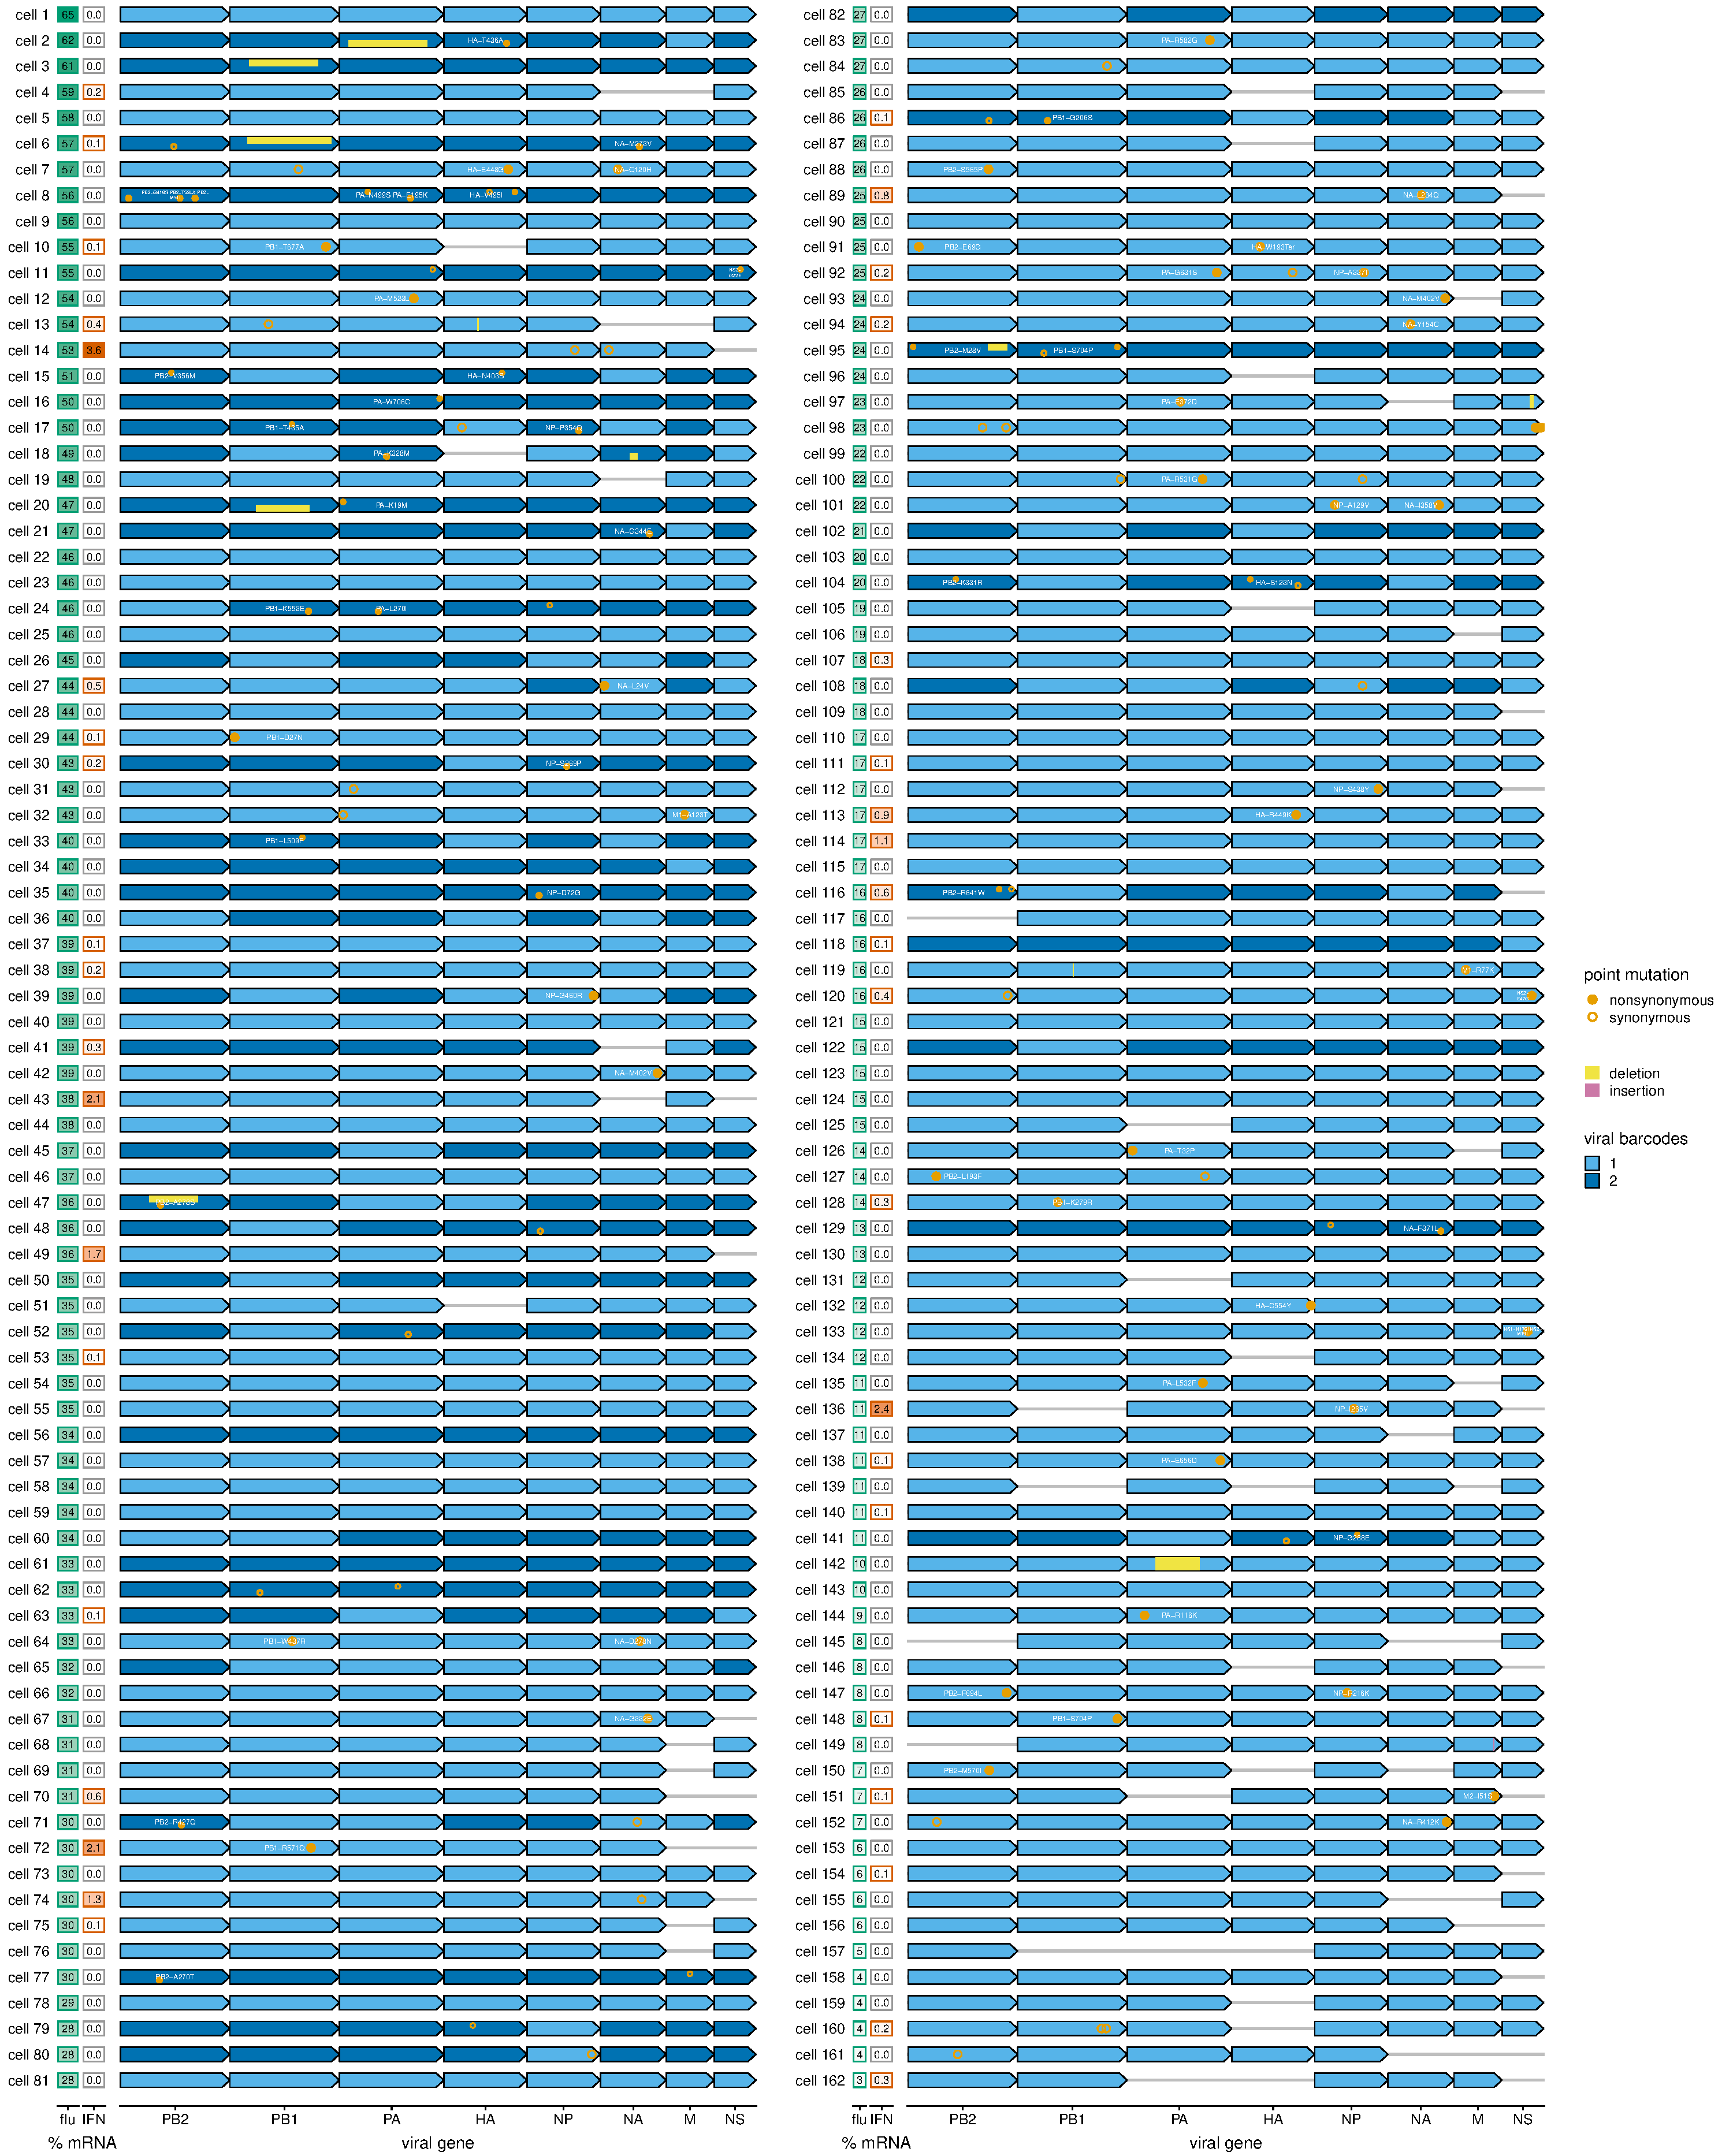
\includegraphics[width=0.9\linewidth]{figures/p_genotypes.pdf}
}
\caption{Viral genotypes and infection outcomes in single cells.}
\label{fig:genotypes}

\figsupp[Genotypes and infection outcomes plotted separately for IFN+ and IFN- cells.]
{This plot shows the same data as \FIG{genotypes}, but with cells separated into columns based on whether they are IFN- or IFN+.}
{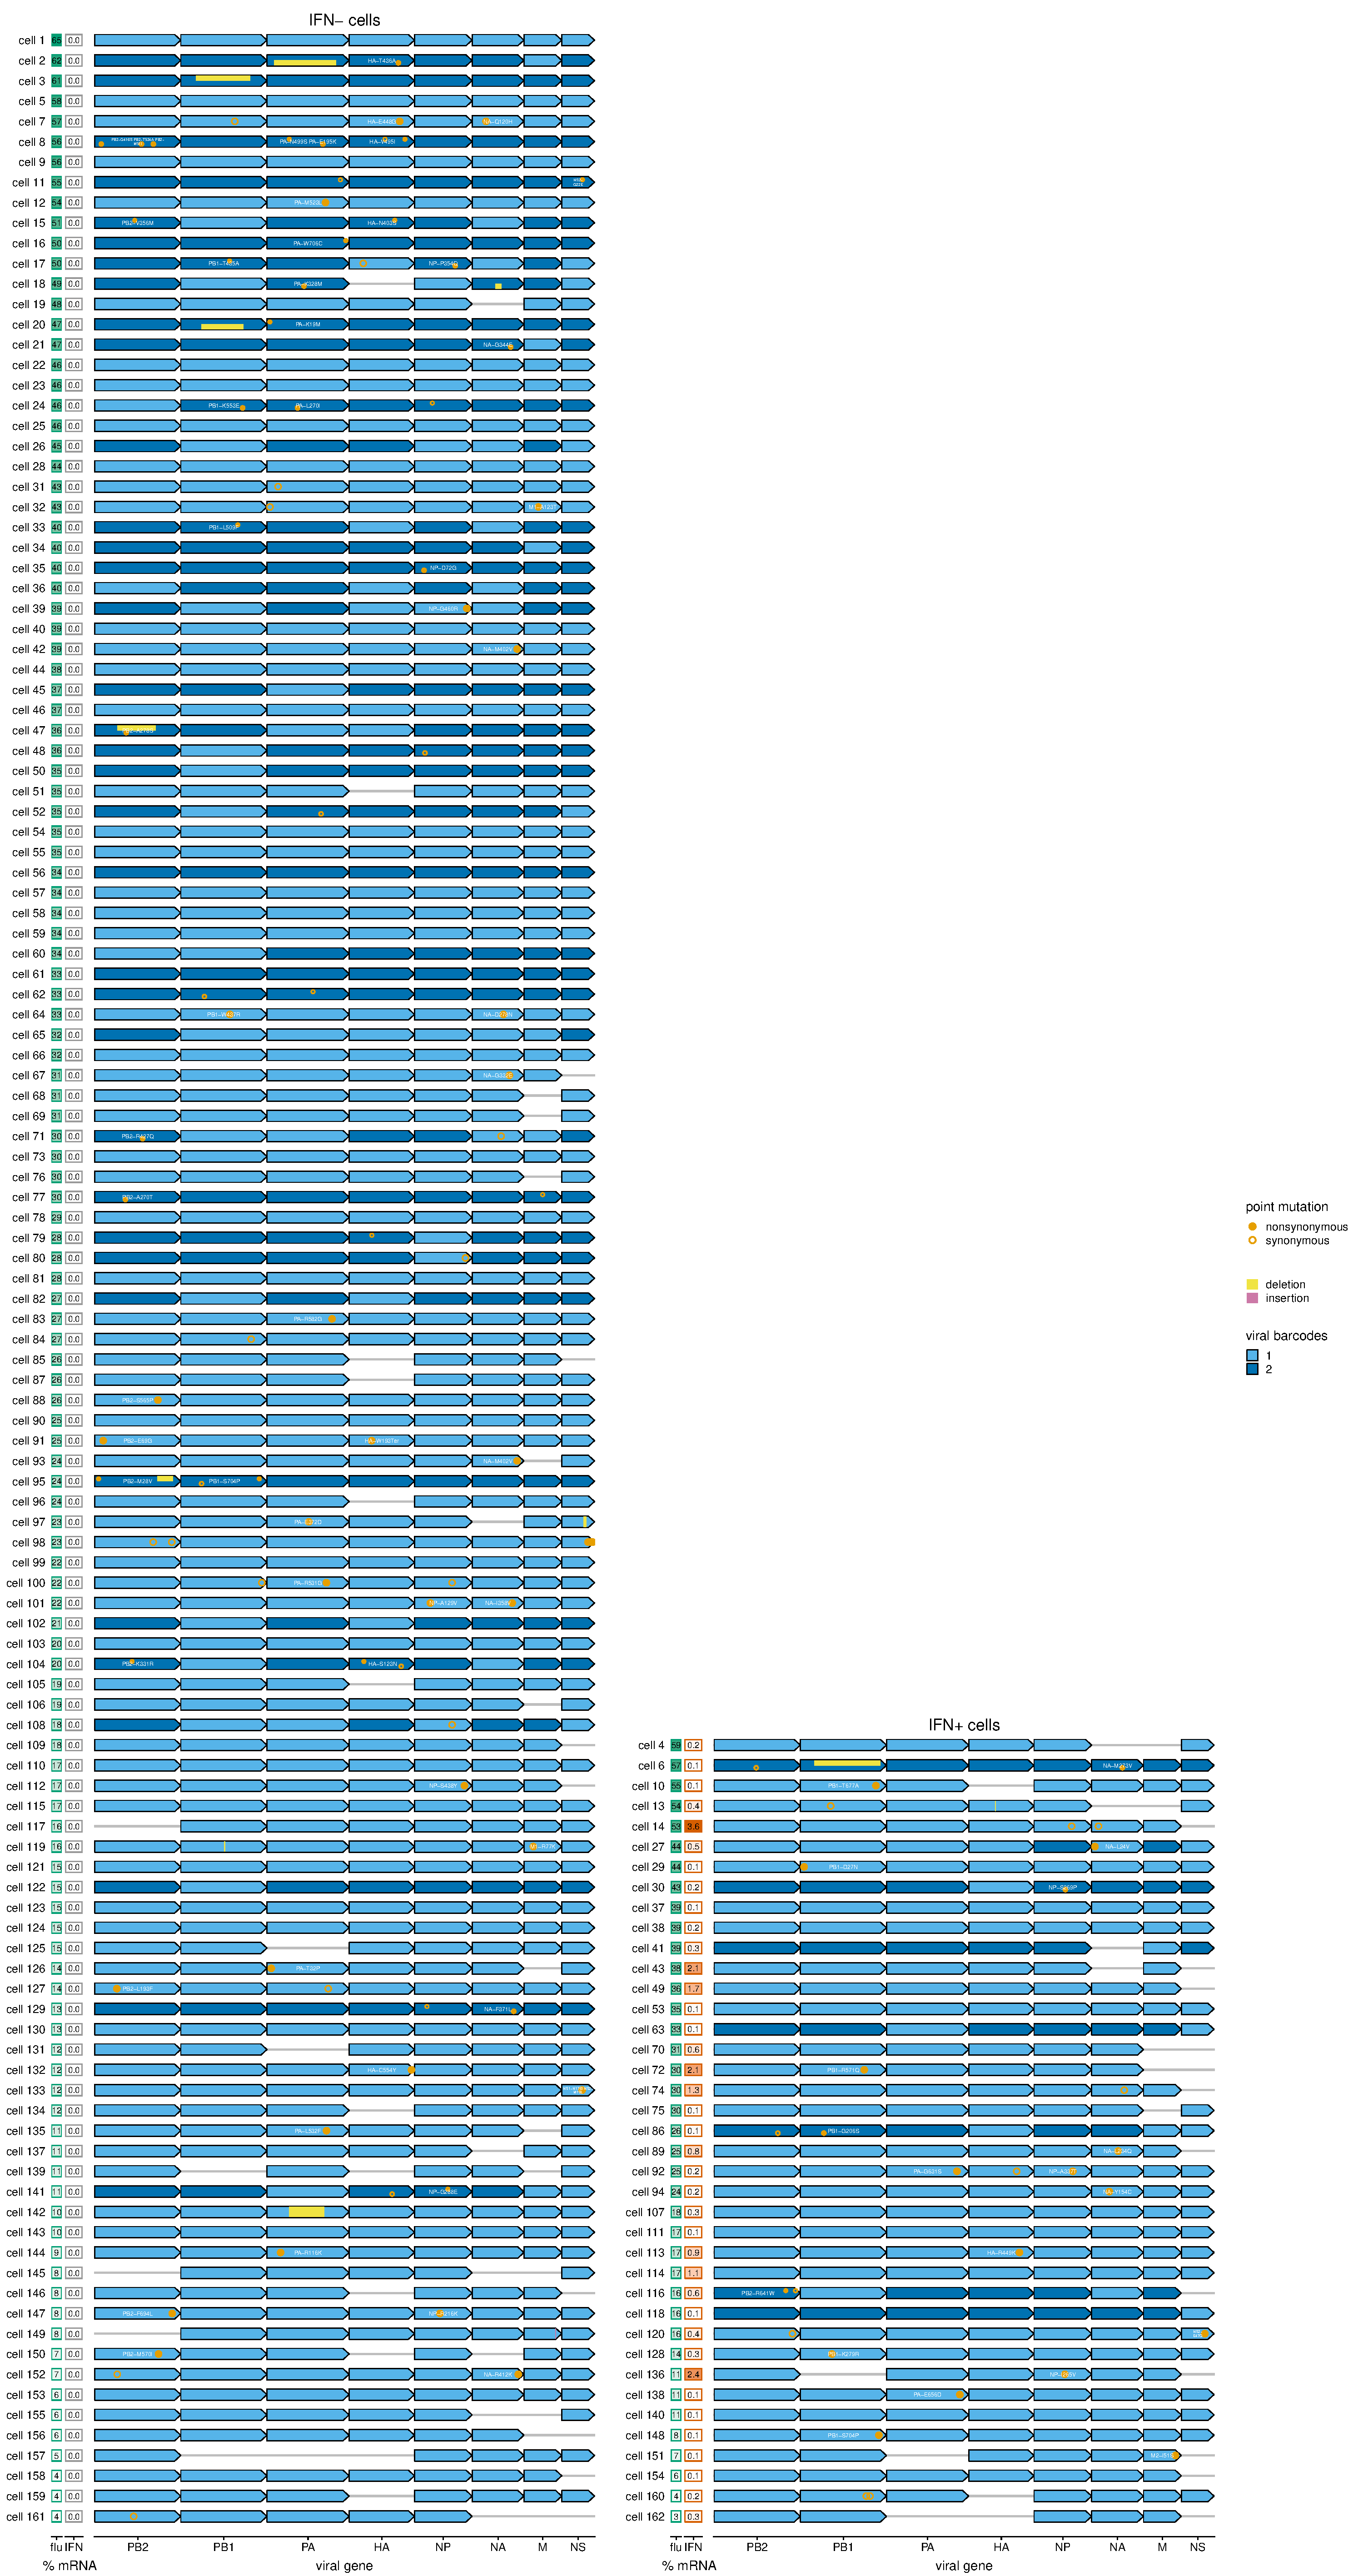
\includegraphics[height=0.95\textheight]{figures/p_genotypes_by_ifn.pdf}}
\label{figsupp:genotypes_by_ifn}

\figdata{A CSV file giving the genotypes is in \texttt{figures/genotypes.csv}.}
\label{figdata:genotypes}

\end{fullwidth}
\end{figure}

\section{Discussion}

Add text

\section{Methods and Materials}

Add text




\section{Acknowledgments}

Add this

\nolinenumbers

\bibliography{references}

\end{document}
